\documentclass{beamer}
\usepackage{pgfpages}
\usepackage{amsmath}
\usepackage{tikz}
\usetikzlibrary{shapes.geometric}
\usetikzlibrary{positioning}
%\pgfpagesuselayout{4 on 1}[a4paper,border shrink=5mm,landscape]

% \usetheme{Warsaw}
% \usecolortheme{crane}
\useinnertheme{rectangles}
\useoutertheme{tree}
\usefonttheme{serif}

\title{Basic Trig func}
\subtitle{Using Beamer}
\author{Nasif}
\institute{BUET}
\date{\today}

\tikzset{darkstyle/.style={circle,draw,fill=gray!40}}

\begin{document}

\section{Introduction}

\begin{frame}
    \titlepage
\end{frame}

\begin{frame}{Trigonometric Identities}
    Quotient Identities
    \[ \tan{\theta} = \frac{\sin{\theta}}{\cos{\theta}} \quad \cot{\theta} = \frac{\cos{\theta}}{\sin{\theta}} \]

    Reciprocal Identities
    \[
    \sin{\theta} = \frac{1}{\csc{\theta}}
    \quad
    \cos{\theta} = \frac{1}{\sec{\theta}}
    \quad
    \tan{\theta} = \frac{1}{\cot{\theta}}
    \]
    Pythagorean Identities
%%%%%%%%%%%%%%
\end{frame}

\begin{frame}{Where did our pytharorean identities come from?}
\Large{Do you remember unit circle?}
    \begin{itemize}
        \item what is the eqn of unit circle?
        \pause
        \[
    x^2+y^2=1
        \]
        \item what does x mean and what does y?
        \pause
        \[
    \sin{\theta}^2+\cos{\theta}^2=1
        \]
        \pause
        %%%%%%%
        Pythagorean identity
    \end{itemize}
\end{frame}

\begin{frame}{Using the identities you now know, find the trig value}
    \begin{enumerate}
    \begin{columns}
        \column{0.5\textwidth}
        % \begin{enumerate}
        
            \item if $\cos{\theta}=\frac{3}{4}$, find $\sec{\theta}$
            \pause
        \[
    \sec{\theta}=\frac{1}{\cos{\theta}}=\frac{4}{3}
            \]
        % \end{enumerate}
    \pause
        \column{0.5\textwidth}
        \item if $\cos{\theta}=\frac{3}{5}$, find $\csc{\theta}$
    \end{columns}
    %%%%%%%%%%%%%%%%%%%%%%%%%%%%%%%%%%%%%%%%
    \end{enumerate}
\end{frame}

\begin{frame}{Simplify each expression}
    \begin{columns}
        \column{.33\textwidth}
        \[
    \frac{\csc{\theta}}{\cot{\theta}}
        \]
        \onslide<2-> derivation
        \column{.33\textwidth}
        \onslide<1->
        \[
    \cos{\theta} \csc{\theta} \tan{\theta}
        \]
        \onslide<3-> derivation
        \column{.33\textwidth}
        \onslide<1->
        \[
    \cos{\theta} \cot{\theta} + \sin{\theta}
        \]
        \onslide<4-> derivation
    \end{columns}
\end{frame}

\begin{frame}{Example}
Simplify
\[ 
    \csc^2{x} \cot{x} \- \cot{x} \]
    \onslide<2->
    \[
      = \csc^2{x} \cot{x} \- \cot{x}
     \]
     \onslide<3->
    \[
      = \csc^2{x} \cot{x} \- \cot{x}
     \]

    
\end{frame}

\begin{frame}{PRACTICE}
\begin{tabular}{|c|c|c|c|}
\hline
    sin & cos & tan & csc \\
     \hline
     & & &  \\
     \hline
     & & &  \\
     \hline
     & & &  \\
     \hline
      
\end{tabular}
    
\end{frame}

\begin{frame}
% \begin{tikzpicture}[]
% % \draw (0:0) -- (0:3);
% % \draw (0:0) -- (60:3);
% % \draw (0:0) -- (120:3);
% % \draw (0:0) -- (180:3);
% % \draw (0:0) -- (240:3);
% % \draw (0:0) -- (300:3);


% % \draw (300:3) -- (0:3);
% % \draw (0:3) -- (60:3);
% % \draw (60:3) -- (120:3);
% % \draw (120:3) -- (180:3);
% % \draw (180:3) -- (240:3);
% % \draw (240:3) -- (300:3);

% % \node [right] at (0:3) {A};
% % \node [above] at (60:3)  {A};
% % \node [above] at  (120:3) {A};
% % \node [left] at  (180:3) {A};
% % \node [below] at  (240:3)  {A};
% % \node [below] at  (300:3)  {A};


% \end{tikzpicture}

    \begin{center}
        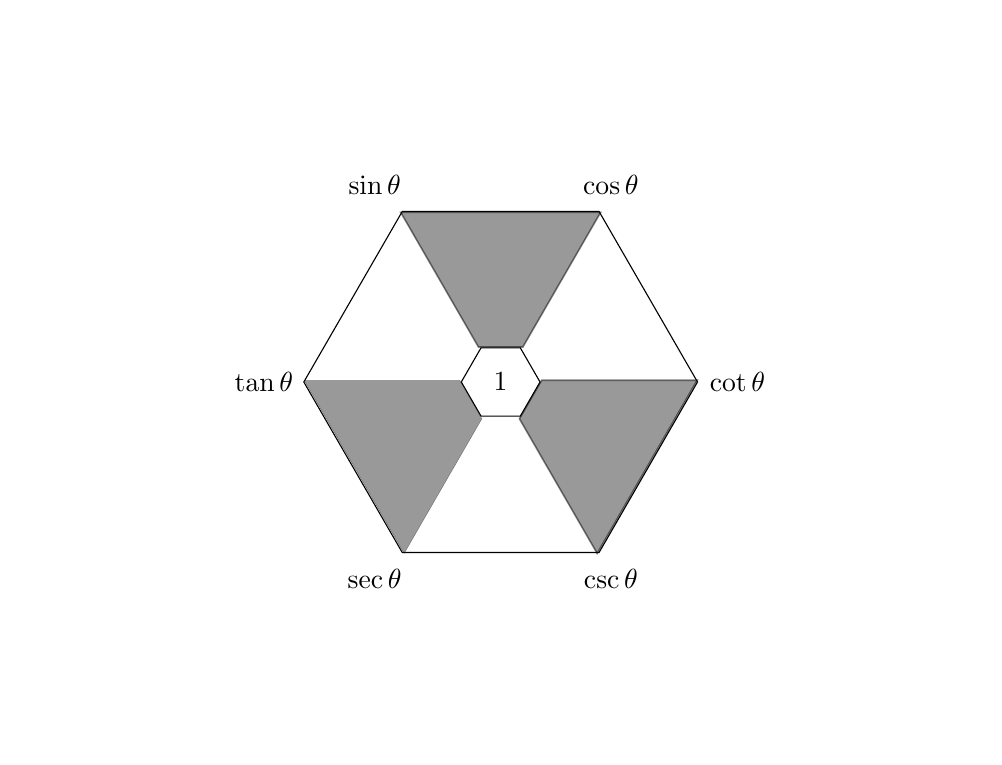
\begin{tikzpicture}[minimum width = 6cm, minimum height = 4cm]
            \node[regular polygon,
            minimum size=5cm,
            draw,
            regular polygon sides = 6,] (p) at (0,0) {}
            node[left] {$\tan\theta$}
            node[right] {$\cot\theta$}
            node at (-1.6, 2.5) {$\sin\theta$}
            node at (+1.4, 2.5) {$\cos\theta$}
            node at (-1.6, -2.5) {$\sec\theta$}
            node at (+1.4, -2.5) {$\csc\theta$}
            ;
            
            \node[regular polygon,
            minimum size=1cm,
            draw,
            regular polygon sides = 6,] (p_innter) at (0,0) {};

            % \filldraw (1.25,2.15) circle (0.1cm);
            % \filldraw (-1.25,2.15) circle (0.1cm);
            % \filldraw (1.25,-2.15) circle (0.1cm);
            % \filldraw (-1.25,-2.15) circle (0.1cm);

            \node[trapezium,
            draw = black,
            line width=0.2mm,
            minimum width = 3pt, 
            minimum height = 1.71cm,
            inner xsep = 1.1pt,
            fill = black!80,
            opacity = 0.5,
            trapezium angle = -60] (t) at (0,1.3) {};

            \node[trapezium,
            rotate = -60,
            draw = black,
            line width=0.1pt,
            minimum width = 3pt, 
            minimum height = 1.71cm,
            inner xsep = 1.1pt,
            fill = black!80,
            opacity = 0.5,
            trapezium angle = 60] (t) at (-1.12,-0.65) {};

            \node[trapezium,
            rotate = 60,
            draw = black,
            line width=0.2mm,
            minimum width = 3pt, 
            minimum height = 1.71cm,
            inner xsep = 1.1pt,
            fill = black!80,
            opacity = 0.5,
            trapezium angle = 60] (t) at (1.12,-0.65) {};

            \node at (0, 0) {1};
        \end{tikzpicture}
    \end{center}

\end{frame}


\begin{frame}
    \begin{center}
        \begin{tikzpicture}
            \node[regular polygon,
            minimum size=5cm,
            draw,
            regular polygon sides = 6,] (p) at (0,0) {}
            node at(0:3) {$\cot\theta$}
            node at (60:3) {$\cos\theta$}
            node at (120:3) {$\sin\theta$}
            node at (180:3) {$\tan\theta$}
            node at (240:3) {$\sec\theta$}
            node at (300:3) {$\csc\theta$}
            ;
            
            \node[regular polygon,
            minimum size=1cm,
            draw,
            regular polygon sides = 6,] (p_innter) at (0,0) {};

            \node at (0, 0) {1};

            \draw [thick] (300:0.5) -- (300: 2.5);
            \draw [thick] (0:0.5) -- (0: 2.5);
            \draw [thick] (60:0.5) -- (60: 2.5);
            \draw [thick] (120:0.5) -- (120: 2.5);
            \draw [thick] (180:0.5) -- (180: 2.5);
            \draw [thick] (240:0.5) -- (240: 2.5);

            \foreach \i in {60, 180, 300}{
                \pgfmathtruncatemacro{\s}{\i}
                \pgfmathtruncatemacro{\e}{\i + 5}
                \node [fill=gray] 
                (\s) -- (\e:2.5) 
                -- (\e:0.5) -- (\s:0.5) -- cycle;
            }
            % \draw [fill=gray] 
            % (300:2.5) -- (0:2.5) 
            % -- (0:0.5) -- (300:0.5) -- cycle;
        \end{tikzpicture}
    \end{center}

\end{frame}

\begin{frame}
    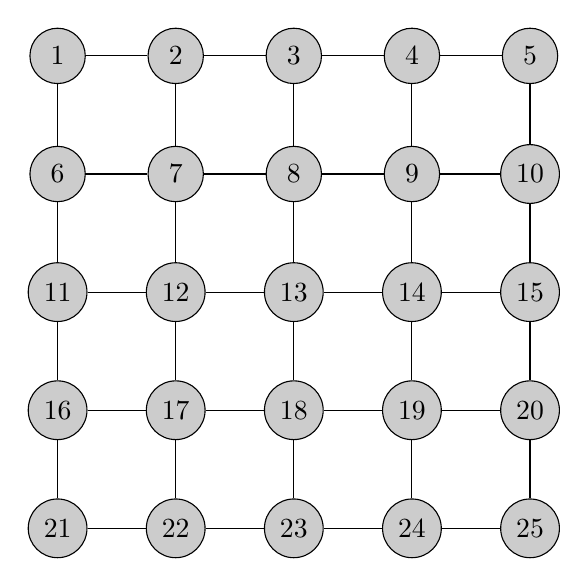
\begin{tikzpicture}
        \foreach \i in {1,...,25}
        {
            \pgfmathtruncatemacro{\y}{(\i - 1) / 5}
            \pgfmathtruncatemacro{\x}{\i - 5 * \y}
            \pgfmathtruncatemacro{\label}{\x + 5 * (4 - \y)}
            \node[darkstyle,minimum size=20] (\label) at (1.5*\x,1.5*\y)
            {\label};
        }
        
        % Horizontal connections
        
        \foreach \x in {1,...,4}
        \foreach \y in {0,...,4}
        {
               \pgfmathtruncatemacro{\cur}{\x + 5* \y}
               \pgfmathtruncatemacro{\next}{\cur + 1}
               \draw (\cur) -- (\next);
        }
        
        % Vertical connections
        \foreach \start in {1,...,20}
        {
            \pgfmathtruncatemacro{\down}{\start+5}
            \draw (\start) -- (\down);  
        }
    \end{tikzpicture}
\end{frame}

\end{document}

